\section{Resultados obtidos}

Cada um dos métodos de implementação foram testados com três quantidades de memória distintas, cada qual com três polinômios geradores. A quantidade de memória de cada máquina de estados e os respectivos polinômios geradores estão representados na Tabela \ref{table:genpol}.

\begin{table}[H]
	\centering
	\captionsetup{font=scriptsize}
	\captionof{table}{Representação octal dos polinômios geradores utilizados para gerar os códigos com taxa $1/3$\label{table:genpol}} \label{tab:title2}
	\begin{tabular}{c|ccc}
		\textbf{$m$} & \textbf{$g_{1}(D)$} & \textbf{$g_{2}(D)$} & \textbf{$g_{3}(D)$} \\ \hline
		3 & 13 & 15 & 17 \\
		4 & 25 & 33 & 37 \\
		6 & 117 & 127 & 155
	\end{tabular}
\end{table}

\subsection{Máquina de estados com 3 memórias}

O resultado obtido para a máquina de estados com 3 memórias está representado na Figura \ref{fig:Fig1aM}.

\begin{figure}[H]
\centering
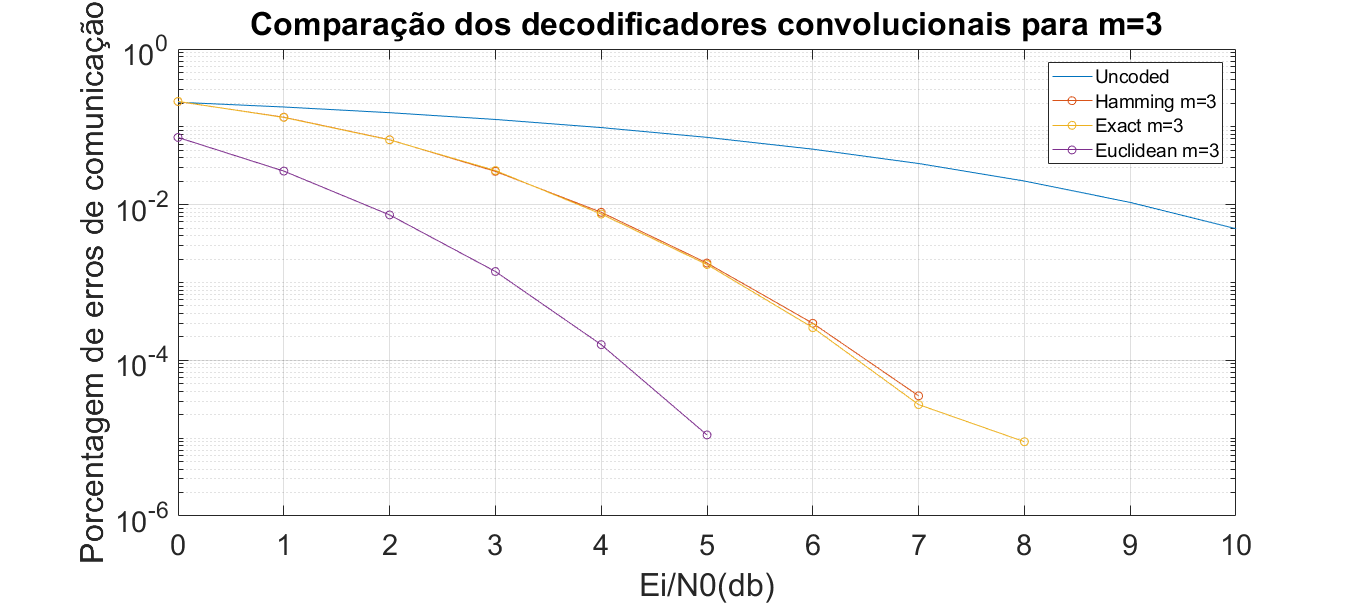
\includegraphics[width=9cm]{Fig1aM}
\captionsetup{font=scriptsize}
\caption{Gráfico da porcentagem de erro pela razão sinal ruído normalizada para m=3\label{fig:Fig1aM}}
\end{figure}

\subsection{Máquina de estados com 4 memórias}

O resultado obtido para a máquina de estados com 4 memórias está representado na Figura \ref{fig:Fig1bM}.

\begin{figure}[H]
	\centering
	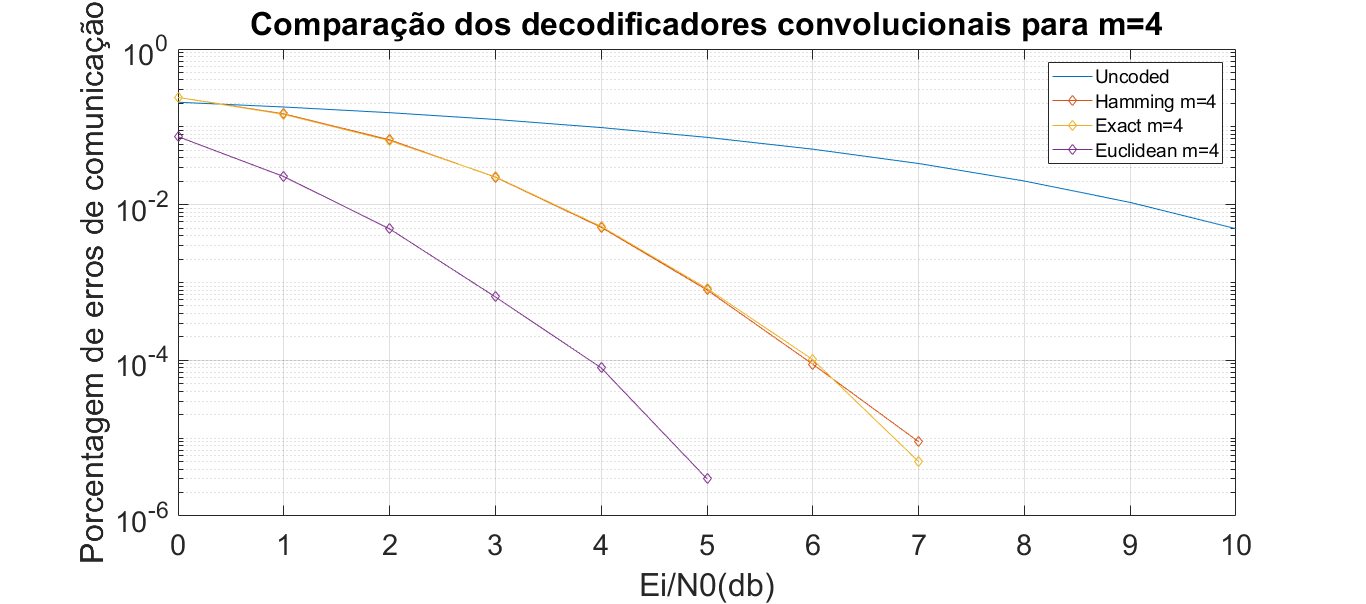
\includegraphics[width=9cm]{Fig1bM}
	\captionsetup{font=scriptsize}
	\caption{Gráfico da porcentagem de erro pela razão sinal ruído normalizada para m=4\label{fig:Fig1bM}}
\end{figure}

\subsection{Máquina de estados com 6 memórias}

O resultado obtido para a máquina de estados com 6 memórias está representado na Figura \ref{fig:Fig1cM}.

\begin{figure}[H]
	\centering
	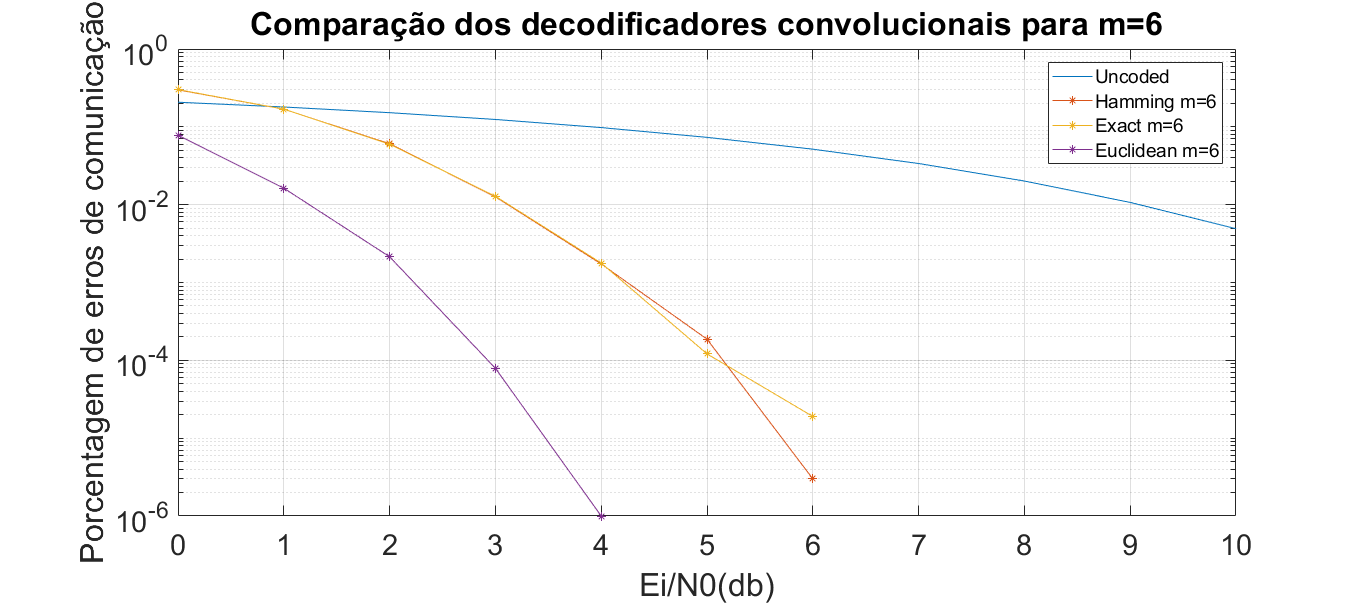
\includegraphics[width=9cm]{Fig1cM}
	\captionsetup{font=scriptsize}
	\caption{Gráfico da porcentagem de erro pela razão sinal ruído normalizada para m=6\label{fig:Fig1cM}}
\end{figure}